\chapter{Results}
\label{ch:results}

This chapter shows what our reconstruction does to aberrated scenes. For four scenes, two under eyedrop gel and two in chicken-breast tissue, we place the regular-camera image next to the global-stage average $G$ and the final rectified image $I_{\mathrm{rect}}$ of one run. We then follow how the blur changes from one image to the next. We chose the scenes by eye and set the reconstruction parameters for each run separately.

\draftnote{\textbf{PREFACE, SAMPLES AND EVALUATION (from the former Chapter~4, \texttt{04\_our\_setup.tex}, removed 2026-11-25, text in Git history at \texttt{f4826a7}; author and supervisor decisions, 2026-11-24; moved here from the Chapter~3 B2--B3 notes on 2026-11-25).} \textbf{Preface} (a short section inside the 6 pages; the supervisor: ``two lines''): the regular camera and the light-field camera and how both see the sample (a flip mirror before the lenslet array sends the light to the regular camera, so its image is captured at a different time from the light-field image), and 488~nm excitation, matched to the absorption of the beads: Thermo Fisher Invitrogen FluoSpheres carboxylate-modified, 2.0~$\mu$m, yellow-green (505/515), F8827 (bibliography entry still to add). Not in the body: the laser model and power, beam expanders, lens part numbers and separations, the excitation coupling, the camera filters, and the Validation Camera (appendix only). \textbf{Samples:} no sample section; each results subsection (tissue, eyedrop gel) opens with what the sample is and where its aberration comes from. For the eyedrop specimen of June~3, 2026: beads diluted, dried on a slide and covered with Systane gel; the unrecorded quantities (dilution convention, drop thickness, coverglass) in one clause or in the appendix. \textbf{Evaluation:} no separate section; it is explained through the results. The primary comparison is within one run: the global-stage average against the final rectified image, same region, boundaries excluded; comparisons with an external camera need registration and carry the sample-change caveat. \textbf{To the appendix} (system details and acquisition records, not yet created): the archive table, the reconstruction and selection records, the dark-frame and exposure-fusion remarks, the full evaluation protocol, and the capture labels, exposure, gain and timing. Source text: \texttt{04\_our\_setup.tex}.
\textbf{Status (2026-11-25):} the preface is drafted as \cref{sec:imaging-setup} (about 125 words) and revised after author review: the regular image's role is the conventional-microscope comparison; both cameras record fluorescence only (the emission filters are mounted on the Fourier lens, before the flip mirror); no sample-change caveat (author: obvious from the flip mount and not relevant for these samples). Spectrum cited from the Thermo Fisher F8888 page (yellow-green, 505/515), which does not mention 488~nm, so the text says 488~nm is near the 505~nm peak rather than claiming a band. \textbf{Status (2026-11-26):} the opening and \cref{sec:results-eyedrop} are drafted (plan: \texttt{planning/05-results-plan.md}); the tissue section and the closing are next.}

\section{Imaging setup}
\label{sec:imaging-setup}

% Drafted 2026-11-25 from the former Chapter 4 (04_our_setup.tex, removed 2026-11-25; Optical configuration) and research-context/physical-system-composition.md. Body facts only; the laser model, coupling, filters and Validation Camera are for the appendix.
We imaged every sample with the instrument of \cref{sec:design-parameters}, using two cameras behind the same objective. A flip mirror before the lenslet array selects the camera. Through the array, the light reaches the light-field camera, which records the views; through a single lens instead, it reaches a regular camera, which records a conventional image of the same field (\cref{sec:conventional-reminders}). Emission filters before the mirror pass only fluorescence to both cameras. We compare each reconstruction with the regular camera's image of the same scene, registered to it, as the capture of a conventional microscope.

The samples are excited at 488~nm through the same objective. All of them contain 2.0~$\mu$m yellow-green fluorescent beads (Thermo Fisher FluoSpheres), excited near their 505~nm maximum and emitting at 515~nm \cite{thermofisher2026fluospheresYellowGreen}, the wavelength used in the design of Chapter~\ref{ch:light-field-microscope}.



\section{Beads under eyedrop gel}
\label{sec:results-eyedrop}

% Drafted 2026-11-26 (planning/05-results-plan.md). Observations only; interpretation belongs to Chapter 6.
We built the first sample to make the aberration change as much as possible within one capture. A single large drop of Systane gel eyedrops covers a layer of beads dried on a microscope slide (\cref{sec:app-samples}). The drop is dome-shaped, so light from beads at different positions leaves the gel through surfaces of different tilt and thickness, and this change is fastest near the edge of the drop. We therefore imaged fields close to the edge, aiming to capture beads both under the gel and beyond it. Over a field of about 0.5~mm this is not quite possible, but the aberration still varies strongly from one side of the field to the other. We show two such fields.

The regular-camera image of the first field (\cref{fig:trio-eyedrop-dense6}, left) shows what a conventional microscope records here. Most beads appear as arcs or streaks rather than spots. Near the top of the field, each bead is spread into a faint dome-shaped arc, while near the bottom the arcs shrink into short bright streaks. The transition between the two roughly follows a curve across the image, which we attribute to the edge of the drop. The blur thus changes shape from one region to the next, and no single blur describes the whole image.

Aligning each view by one shift already changes this picture. In the global-stage average $G$ (middle), most arcs and streaks collapse into compact spots, in the upper and lower parts of the field alike. What remains are places where one shift per view could not bring all the copies of a bead together. The orange inset is one of them: $G$ shows a single elongated patch where the regular camera shows two overlapping blurs, visible only on the lower display window of its second inset. After local refinement, the same patch appears in the final rectified image $I_{\mathrm{rect}}$ (right) as three distinct spots. In the cyan inset, where $G$ already shows four separate spots, local refinement only makes them slightly more compact.

\begin{figure}[t]
    \centering
    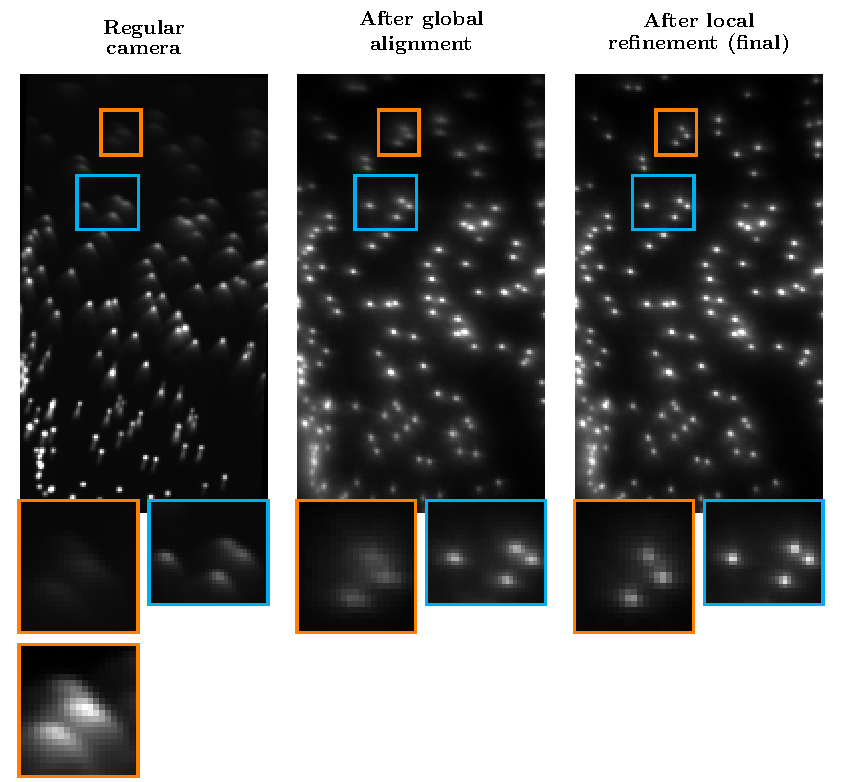
\includegraphics[width=0.9\linewidth]{figures/ch05/trio-eyedrop-dense6.pdf}
    \caption[Beads under eyedrop gel, first field.]{Beads under eyedrop gel, first field (dense6). Left to right: the regular-camera image, downsampled and registered to the reconstruction; the global-stage average $G$; and the final rectified image $I_{\mathrm{rect}}$, both from one reconstruction run. The insets below each column enlarge the orange and cyan regions. $G$ and $I_{\mathrm{rect}}$ share one linear display window (200.6 to 8853 counts), and the regular-camera image has its own (0 to 3550 counts). The lower orange regular-camera inset is rescaled to 101.4 to 478.8 counts to show the faint beads and is not comparable in brightness. No smoothing, background subtraction or gamma was applied.}
    \label{fig:trio-eyedrop-dense6}
\end{figure}

In the second field (\cref{fig:trio-eyedrop-dense7}), the arcs are larger and the regular camera loses more. Toward the bottom of the image, the arcs of neighboring beads merge into bright streaks in which single beads cannot be told apart (cyan inset), and here too the change in blur follows a curved band across the field. In $G$, the same region already becomes a group of separate spots around one bright bead. Local refinement then tightens the bright bead and its neighbors. In the orange inset, four faint beads that form overlapping arcs in the regular image appear as small spots in $G$ and as slightly tighter ones in $I_{\mathrm{rect}}$.

\begin{figure}[t]
    \centering
    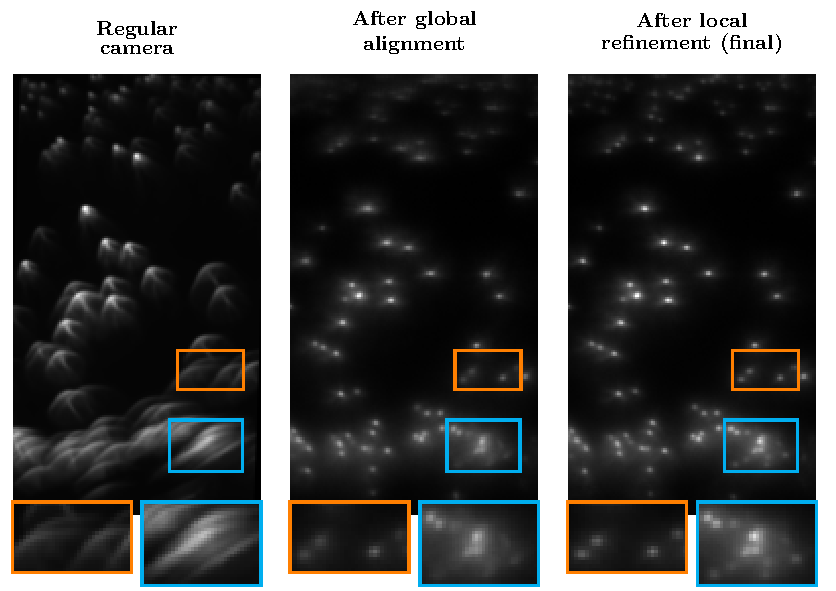
\includegraphics[width=0.9\linewidth]{figures/ch05/trio-eyedrop-dense7.pdf}
    \caption[Beads under eyedrop gel, second field.]{Beads under eyedrop gel, second field (dense7). Columns and insets as in \cref{fig:trio-eyedrop-dense6}. $G$ and $I_{\mathrm{rect}}$ share one linear display range, from the minimum to the maximum of the two images (152 to 13407 counts), and the regular-camera image is scaled linearly from its own minimum to its maximum. No smoothing, background subtraction or gamma was applied.}
    \label{fig:trio-eyedrop-dense7}
\end{figure}

In both fields, the two stages divide the work in the same way. Global alignment does most of the correction, turning arcs and streaks into spots across the whole field. Local refinement then acts only where one shift per view is not enough: spots that are elongated or merged in $G$ become compact or separate in $I_{\mathrm{rect}}$, while isolated spots change little. Since $G$ and $I_{\mathrm{rect}}$ average the same views of the same run, these differences come from the local stage alone. Note that the comparison with the regular camera concerns the shape of the blur rather than the finest detail, since every view, and with it $G$ and $I_{\mathrm{rect}}$, is limited to the resolution $\Delta x_{LF}=N\Delta x_o$ of \cref{eq:lateral-lf}.

In the gel, the aberration comes from the shape of one smooth surface above the beads. In the second sample, it comes from the tissue itself.
